\documentclass[../main.tex]{subfiles}
%!TEX root = ./appendixFromAnalysisDossier.tex
\graphicspath {{../}}

\begin{document}
\section{Vectoring Motor} \label{vectoringMotor}
In order to determine the required torque of the servo that is at the end  of the thruster shaft, worst case scenario moments of inertia were considered, as seen in Figure \ref{fig:ThrusterI}. The angular acceleration can be set for any chosen servo motor as long as the acceleration is less than the specified maximum. The shaft could be either hollow or solid, therefore the solid case was chosen to account for the higher moment of inertia. The thruster motor and mounting bracket were considered as a single rectangular prism. The propeller was also considered as a rectangular prism.

\begin{equation}
T_{servo} = I_{total}\cdot{}\alpha
\end{equation}

\begin{equation}
I_{total} = \frac{m_{shaft}\cdot{}r_{st}^2}{2} + \frac{(m_{motor} + m_{bracket})}{12} \cdot{}(d_{m_{x}}^2 + d_{m_{z}}^2) + \frac{m_{prop}}{12}\cdot{}(d_{p+{x}}^2 + d_{p_{z}}^2)
\end{equation}

\begin{figure}[H]
	\centering
	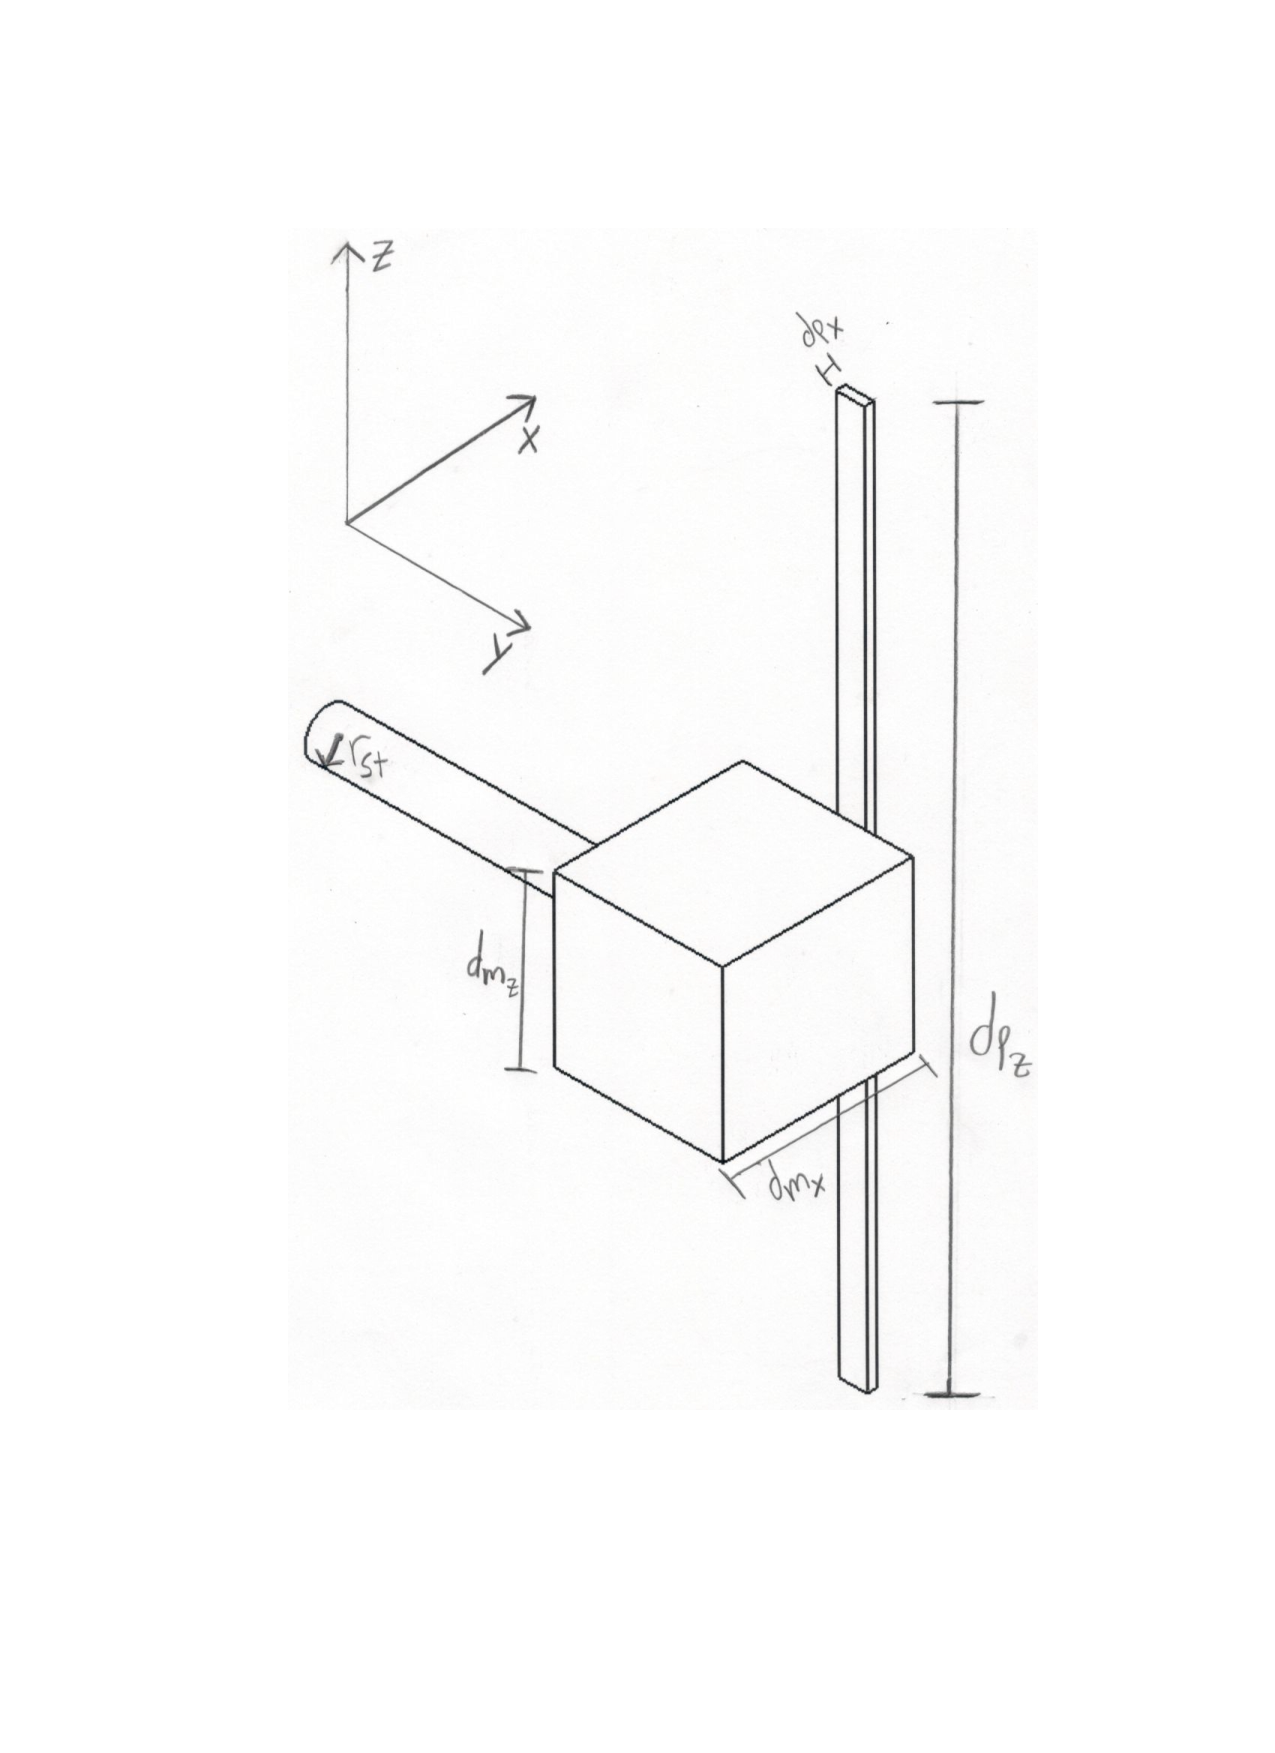
\includegraphics[width=0.5\textwidth]{img/analysis/thruster/thruster1.pdf}
	\caption{Thruster Pitching Shaft Worst Case Moment of Inertia}
	\label{fig:ThrusterI}
\end{figure}

\end{document}